In the sequel we assume that $L_1 = L_2 = \dots = L_t \triangleq L$  in the surveillance game structure, i.e, all $n$ sensors and the target operate in the same state space. For the remainder of the paper, let $G=(\states,s^\init,\trans,\vis_1,\ldots,\vis_n)$ be a multi-agent surveillance game structure  defined over  $L$, and let $\mathcal M = \{\Lambda_1,\dots,\Lambda_m\}$ be a set of static sensors. We define a  \emph{state-space partition} of size $n$ of the set $L$ of locations in a game structure $G$ to be a tuple $\widetilde L =  (\widetilde L_1,\ldots,\widetilde L_n)$ of subsets of $L_i$ such that  $\bigcup_i^n \widetilde L_i = L $, and $\widetilde L_i \cap \widetilde L_j  = \emptyset$ for $i \neq j$. 


\begin{figure}
\subfloat[Multi-agent surveillance game partitioned into two subgames. \label{part-grid}]{
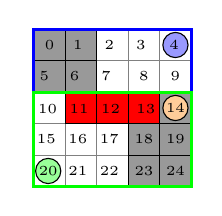
\begin{tikzpicture}[scale=0.8]
\draw[step=0.5cm,color=gray] (-1.5,-1.5) grid (1,1);
\filldraw[fill=red,draw=black] (0,0) rectangle (-0.5,-0.5);
\filldraw[fill=red,draw=black] (-0.5,0) rectangle (-1,-0.5);
\filldraw[fill=red,draw=black] (0,0) rectangle (0.5,-0.5);
\filldraw[fill=gray!80!white,draw=black] (-0.5,0.5) rectangle (-1,1);
\filldraw[fill=gray!80!white,draw=black] (-0.5,0) rectangle (-1,0.5);
\filldraw[fill=gray!80!white,draw=black] (-1,0.5) rectangle (-1.5,1);
\filldraw[fill=gray!80!white,draw=black] (-1,0) rectangle (-1.5,0.5);
\filldraw[fill=gray!80!white,draw=black] (0.5,-0.5) rectangle (1,-1);
\filldraw[fill=gray!80!white,draw=black] (0,-0.5) rectangle (0.5,-1);
\filldraw[fill=gray!80!white,draw=black] (0,-1) rectangle (0.5,-1.5);
\filldraw[fill=gray!80!white,draw=black] (0.5,-1) rectangle (1,-1.5);
\filldraw[fill=gray!80!white,draw=black] (0.5,-0.5) rectangle (1,0);

\filldraw[fill=blue!40!white,draw=black] (+0.75,+0.75) circle (0.2cm);
\filldraw[fill=orange!40!white,draw=black] (0.75,-0.25) circle (0.2cm);
\filldraw[fill=green!40!white,draw=black]  (-1.27,-1.25) circle (0.2cm);
\filldraw[fill=none,draw=blue,line width=0.4mm] (-1.5,0) rectangle (1,1);
\filldraw[fill=none,draw=green,line width=0.4mm] (-1.5,-1.5) rectangle (1,0);
\node at (-1.25,+0.75) {\tiny{0}};
\node at (-0.80,+0.75) {\tiny{1}};
\node at (-0.30,+0.75) {\tiny{2}};
\node at (0.20,+0.75) {\tiny{3}};
\node at (0.73,+0.75) {\tiny{4}};
\node at (-1.33,+0.25) {\tiny{5}};
\node at (-0.85,+0.25) {\tiny{6}};
\node at (-0.35,+0.25) {\tiny{7}};
\node at (0.25,+0.25) {\tiny{8}};
\node at (0.75,+0.25) {\tiny{9}};
\node at (-1.28,-0.27) {\tiny{10}};
\node at (-0.78,-0.27) {\tiny{11}};
\node at (-0.28,-0.27) {\tiny{12}};
\node at (0.28,-0.27) {\tiny{13}};
\node at (0.75,-0.25) {\tiny{14}};
\node at (-1.3,-0.75) {\tiny{15}};
\node at (-0.8,-0.75) {\tiny{16}};
\node at (-0.3,-0.75) {\tiny{17}};
\node at (0.25,-0.75) {\tiny{18}};
\node at (0.75,-0.75) {\tiny{19}};
\node at (-1.27,-1.25) {\tiny{20}};
\node at (-0.8,-1.25) {\tiny{21}};
\node at (-0.3,-1.25) {\tiny{22}};
\node at (0.25,-1.25) {\tiny{23}};
\node at (0.75,-1.25) {\tiny{24}};

\end{tikzpicture}
\hspace{.3cm}}
%\hfill
\subfloat[Transitions from initial state in subgames. \label{part-grid-trans}]{

\begin{minipage}{5.0cm}
\vspace{-2.8cm}
%{\fontsize{8}{10}\selectfont $\Vis((20,4),18) = \false,\vis(4,17) = \false,$ $\vis(4,19) = \true, \vis(4,23) = \false$}

%\smallskip

%\small \[\tilde{L} =\begin{cases}
%\widetilde{L}_1 = \{0,1,2,3,4,5,6,7,8,9\} \\
%\widetilde{L}_2 = \{10,11,12,13,14,\ldots,24\}
%
%\end{cases}\]


\begin{tikzpicture}[node distance=.9 cm,auto,>=latex',line join=bevel,transform shape,scale=.75]
\node at (0,0) (s0) {$G^1: (20,14)$};
\node  [below left of=s0,yshift=-.5cm,xshift=-0.5cm] (s2) {$(21,k_1)$};
\node  [below right of=s0,yshift=-.5cm,xshift=0.5cm] (s3) {$(15,k_1)$};
\node  [left of=s2,xshift=-0.75cm] (s1) {$(21,\{19\})$};
\node  [right of=s3,xshift=0.75cm] (s4) {$(15,\{19\})$};
\draw [->] (s0) edge (s1.north);
\draw [->] (s0) edge (s2.north);
\draw [->] (s0) edge (s3.north);
\draw [->] (s0) edge (s4.north);
\end{tikzpicture}



\begin{tikzpicture}[node distance=.9 cm,auto,>=latex',line join=bevel,transform shape,scale=.75]
\node at (0,0) (s0) {$G^2: (4,k_1)$};
\node  [below of=s0,yshift=-.5cm] (s1) {$(3,9)$};
\node  [right of=s1,xshift=0.5cm] (s2) {$(9,k_2)$};
\node  [left of=s1,xshift=-0.5cm] (s3) {$(3,k_2)$};
\draw [->] (s0) edge (s1.north);
\draw [->] (s0) edge (s2.north);
\draw [->] (s0) edge (s3.north);
\end{tikzpicture}



\end{minipage}
}
\hspace{0.2cm}

\caption{Partitioning of the state space of a surveillance game into two subgames with locations $\widetilde{L}_1$ (green) and $\widetilde{L}_2$ (blue). }
\label{fig:simple-dist-game}
\vspace{-0.6cm}
\end{figure}

\subsection{Surveillance Subgames}
We now describe how, given a state-space partition $\widetilde L =  (\widetilde L_1,\ldots,\widetilde L_n)$, to construct a tuple of single-agent surveillance game structures $\widetilde G = (G^1,\ldots,G^n)$ that contains one  \emph{surveillance subgame} $G^i$ for each mobile sensor  $i$. Each subgame, $G^i$ is defined over the subset of locations $\widetilde{L}_i$. Since the target and sensors operate on the same state space we will have $\widetilde{L}^i_s = \widetilde{L}^i_t = \widetilde{L}_i$. Additionally, to each $\widetilde{L}^i_t$ we add an \emph{auxiliary location} $k_i$ that encapsulates all possible locations of the target that are outside of this subgame's region, i.e., all locations in $L \setminus \widetilde{L}_i$.  We then model transitions leaving or entering $\widetilde{L}^i_t$ as transitions to or from location $k_i$ respectively.
We require that the initial location $l_i^\init$ of sensor $i$ is in $\widetilde{L}_i$.

Formally, given a subset  $\widetilde{L}_i \subseteq L$ we define the \emph{subgame} of $G$ corresponding to sensor $i$ as the tuple $G^i = (\widetilde{S}_i,\widetilde{s}_i^{\init},\widetilde{T}_i,\widetilde{\vis}_i)$  where:
\begin{itemize}
\item $\widetilde{S}_i= \widetilde{L}_i \times (\widetilde{L}^i_t \cup k_i)$ is the set of states.
\item $\widetilde s_i^\init = (l_i^\init,\widetilde l_t)$ is the initial state, where $\widetilde l_t =  l_t^\init$, if
$ l_t^\init \in \widetilde L_i$, and $\widetilde l_t = k_i$ otherwise.
\item The set $\widetilde{T}_i$ consists of two types of transitions: the transitions in $T{\downarrow } i$ that originate and end in the subgame's region are preserved as they are. Transitions of the target exiting or entering $\widetilde{L}^i_t$ are replaced by transitions to and from location $k_i$ respectively, since $k_i$ represents all target locations outside of  $\widetilde{L}^i_t$. 
Formally, for every pair of states $(\widetilde{l}_i,\widetilde{l}_t) \in \widetilde{S}_i$ and $(\widetilde{l}_i',\widetilde{l}_t') \in \widetilde{S}_i$ we have that $((\widetilde{l}_i,\widetilde l_t),(\widetilde{l}_i',\widetilde l_t')) \in \widetilde T_i$ if and only if there exists a transition
 $((\widetilde{l}_i,l_t),(\widetilde{l}_i',l_t')) \in T{\downarrow}i$ for which the following conditions are satisfied:
 \begin{itemize}
 \item if $\widetilde l_t \in \widetilde L_t ^i$ and $\widetilde l_t' \in \widetilde L_t ^i$, then 
 $\widetilde l_t = l_t$ and $\widetilde l_t'= l_t'$, that is, we have a \emph{transition internal for the region $\widetilde L_t^i$};
 \item if $\widetilde l_t \in \widetilde L_t ^i$ and $\widetilde l_t' =  k_i$, then 
 $l_t \in \widetilde L_t^i$ and $l_t' \not\in \widetilde L_t^i$, that is, we have a \emph{transition exiting the region $\widetilde L_t^i$}; 
 \item if $\widetilde l_t= k_i$ and $\widetilde l_t' \in  \widetilde L_t ^i$, then 
 $l_t \not \in \widetilde L_t^i$ and $l_t' \in \widetilde L_t^i$, that is, we have a \emph{transition entering the region $\widetilde L_t^i$}; 
 \item if $\widetilde l_t= k_i$ and $\widetilde l_t' =  k_i$, then 
 $l_t \not \in \widetilde L_t^i$ and $l_t' \not\in \widetilde L_t^i$, that is, we have a \emph{transition completely outside $\widetilde L_t^i$}.
\end{itemize}  

  \item The visibility function $\widetilde{\vis}_i$ in the subgame $G^i$ agrees with the visibility function $\vis_i$ of sensor $i$ in the original game when the target's location is in the subgame's region. Target locations outside of the region $\widetilde L_t^i$  (summarized by location $k_i$) are invisible to the sensor in the subgame. Formally, $\widetilde{\vis}_i(\widetilde{l}_i,l_t) = \vis_i(\widetilde{l}_i,l_t)$  when $l_t \in \widetilde{L}_t^i$, and $\false$ if $l_t  = k_i$
% \[\widetilde{\vis}_i(\widetilde{l}_i,l_t) = \begin{cases}
%\vis_i(\widetilde{l}_i,l_t) & \text{if } l_t \in \widetilde{L}_t^i, \\
%\false & \text{if } l_t  = k_i.
%\end{cases}
%\]
\end{itemize}
\begin{example}
In Figure \ref{part-grid}, we have two subgames: $G^1$ for the green mobile sensor and $G^2$ for the blue one. The states in the subgames are $s_1 = (20,14)$, and $s_2 = (4,k_2)$ . Recall that $k_i$ is an indicator state to represent that the target is not subgame $i$. The possible transitions shown in Figure \ref{part-grid-trans} show that the target has the ability to leave $G^1$ and enter $G^2$. 
%Finally recall that in example \ref{ex:simple-surveillance-game}, we had state $Vis((20,4),14) = \true$. This is no longer the case as although we have $\vis_1(4,14) = \true$ in the global game (i.e, it is visible to sensor 1 and hence also visible to the entire sensor network), state 14 does not lie in $\widetilde{L}_1$ which means it is not visible in the subgame for sensor 1.
\qed
\end{example}

Note that in this construction, sensor $i$ is not able to leave the region of locations $\widetilde{L}_i$. Furthermore, all the information about the target's behaviour outside of  the subgame's region is completely hidden from the mobile sensor controller, since all locations outside of  $\widetilde{L}_t^i$ are represented by the single location $k_i$.
%Finally we remark that the previously defined notions of $\succs_t(\widetilde{l}_i,\widetilde{l}^i_{t})$, $\succs_t(\widetilde{l}_i,\widetilde{L}^i_{t})$, and $\succs(\widetilde{l}_i,\widetilde{l}^{t},\widetilde{l}_{t}')$ for the global game structure $G$ follow analogously in this construction for $\widetilde{T}$ which we denote as $\widetilde{\succs}$.
In section \ref{sec:local-games}, we discuss the local knowledge (belief)  of sensor $i$ in the game structure $G^i$.
 
\subsection{Static Sensors in Subgames}
We assumed that all information about the target's behaviour outside of subgame $G^i$ is completely  hidden to sensor $i$. Hence, sensor $i$ is only privy to static sensors that operate in the state space of the subgame $G^i$, i.e, static sensors $\Lambda_m$ where $\Lambda_m \cap \widetilde{L}_i \neq \emptyset$. For simplicity of the presentation we assume that each static static sensor operates in exactly one region $L_i$. Our results can easily be extended to the general case. We define $Q_i = \{i \mid \Lambda_{i} \cap \widetilde{L}_i \neq \emptyset\}$ to be the set of static sensors operating in the subgame  $G^i$. 
%We denote $\widetilde{\Lambda}_q = \Lambda_{q} \cap \widetilde{L}_i$ and define $J_i(\widetilde l_t)\subseteq Q_i$ as the set of triggered static sensors in location $\widetilde l_t \in \widetilde L_i$ in region $i$.

\subsection{Local Beliefs in Surveillance Subgames}\label{sec:local-games}
A surveillance subgame is a game structure with a single mobile sensor and some number of static sensors, and thus, is  a special case of multi-agent surveillance game structure. With this, the definition of  belief-set game structures from Section~\ref{sec:belief-gs} directly applies to surveillance subgames.

In the belief-set game structure for a surveillance subgame $G^{i} = (\widetilde{S}_i,\widetilde{s}_i^{init},\widetilde{T}_i,\widetilde{\vis}_i)$ with static sensors $Q_i$, the belief sets represent the local belief of sensor $i$. More specifically, a belief set in $G^{i}_\belief$ is an element of  $\mathcal{P}(\widetilde{L}^i_t \cup \{k_i\})$, and can thus contain the auxiliary location. Intuitively, if $ k_i$ is present in the sensor's current belief, then the target could possibly be outside of the local set of locations $\widetilde L_i$, or if the belief is the singleton $\{k_i\}$, then sensor $i$ knows for sure that the target is outside of its region. Additionally, if there is a triggered static sensor in the region, the sensor will know that the target must be in the state space of the static sensor and $k_i$ cannot be in the belief.
We define the \emph{global interpretation} $\llbracket B_t\rrbracket$ of a belief set $B_t$ in $G^{i}_\belief$, which is a set of locations in $G$, as
 \[\llbracket B_t\rrbracket = \begin{cases}
B_t & \text{if } k_i \not\in B_t\\
B_t \cup (L \setminus \widetilde L_i) & \text{if } k_i  \in B_t.
\end{cases}
\]
% \[\llbracket B_t\rrbracket = \begin{cases}
%B_t \setminus \bigcup_{q\in Q_i}\tilde{\Lambda}_q & \text{if } k_i \not\in B_t, J_i = %\emptyset \\
%B_t \bigcap_{j\in J_i}\tilde{\Lambda}_j & \text{if } k_i \not\in B_t, J_i \neq \emptyset \\
%B_t \cup (L \setminus \widetilde L_i) & \text{if } k_i  \in B_t.
%\end{cases}
%\]

%belief subgame  $G^{i}_\belief= (\widetilde{\states}_{i_\belief},\widetilde{s}^\init_{i_\belief},\widetilde{\trans}_{i_\belief})$ 
%\begin{itemize}
%\item $\states_{i_\belief} = \widetilde{L}_i \times \mathcal{P}(\widetilde{L}^i_t \cup \{k_i\})$ is the set of states,
%\item $\widetilde{\trans}_{i_\belief} \subseteq \widetilde{\states}_{i_\belief} \times \widetilde{\states}_{i_\belief}$ is the transition relation where $((\widetilde{l}_i, B_t),(\widetilde{l}_i', B_t')) \in \widetilde{\trans}_{i_\belief}$ iff $\widetilde{l}_i' \in  \widetilde{\succs}(\widetilde{l}_i,l_t,l_t')$ for some $l_t \in B_t$ and $l_t' \in B_t'$ and one of these holds:
%\begin{itemize}
%\item[(1)] $B_t' = \{l_t'\}$, $l_t' \in \widetilde{\post}(\widetilde{l}_i,B_t)$, $\widetilde{\vis}_i(l,l_t') = \true$;
%\item[(2)] $B_t' = \{l_t' \in \widetilde{\post}(\widetilde{l}_i,B_t)  \mid  \widetilde{\vis}_i(l,l_t') = \false \}$.
%\end{itemize}
%\end{itemize}
% For brevity, we omit the definitions of $\widetilde{\succs}_t$, $\widetilde{\succs}$, runs and strategies for the belief subgames as the definitions follow trivially from those for the belief games but in the subspace of transitions and states as defined above.

Strategies of sensor $i$ in the belief-set game $G^{i}_\belief$ depend only on the sequence of states in this game, and thus, only on local information. Following the definitions in Section~\ref{sec:belief-gs}, the outcome of a pair of given strategies $f_{i}$ and $f_{t_i}$ for the sensor and the target in $G^{i}_{\belief}$  is a sequence of  states in  $G^{i}_{\belief}$, each of which is a pair consisting of a location of sensor $i$ and a belief-set for sensor $i$ in $G^{i}_{\belief}$.

%\paragraph*{Remark}$B^k_{t_i}$ is the belief that sensor $i$ holds on the position of the target. Since the subgame for each sensor will be executing concurrently, the global belief on the location of the target will be a combination of the knowledge of the individual sensors. This is discussed in more detail in the sequel.

\subsection{Distributed Surveillance Synthesis Problem}\label{sec:distributed-problem}
Given a state-space partitioning $\widetilde L$ and the corresponding tuple of subgames $\widetilde G = (G^1,\ldots,G^n)$
we will define a distributed surveillance strategy synthesis problem, which, intuitively, asks to synthesize strategies for the sensors in the individual belief subgames, such that together they guarantee the global surveillance objective.  In this section we formalize this intuitive problem description. We first need to define what it means for the individual sensor strategies to jointly satisfy together a global requirement.

The surveillance requirements are defined in terms of the belief-states in $G_\belief$, but strategies in the belief subgames are defined in terms of sequences of local belief states. Hence, we need to define a mapping of states of the form $((l_1,\ldots,l_n),B_t,J)$ to elements of $\mathcal{P}(\widetilde{L}^i_t \cup \{k_i\})$ for each $i$. Since, by definition, a strategy for sensor $i$ in the corresponding belief subgame guarantees that it remains in $\widetilde L_i$, we only need to define the mapping for states  $l_i \in\widetilde{L}_i$.

Formally, for a state $((l_1,\ldots,l_n),B_t,J)$  we define its projection on belief subgame $i$ as $((l_1,\ldots,l_n),B_t,J){\downarrow}i = (l_i,B_t{\downarrow}i,J \cap Q_i)$, where
\[B_t{\downarrow}i = \begin{cases}
B_t& \text{if }  B_t \subseteq \widetilde L_i, \\
(B_t \cap \widetilde L_i) \cup \{k_i\} & \text{otherwise}.
\end{cases}\]
The mapping extends to sequences of states in the usual way. 

Intuitively, this mapping projects the joint knowledge of the sensors in $G_\belief$ onto the local belief of each sensor, where the sensors do not share their local beliefs with each other, that is, the sensors have no information about the target's position outside of their own region. The global, shared belief of the sensors is formed by the combination of their local beliefs. More precisely, this is the intersection of the  global interpretation of the local beliefs. Indeed, it is easy to see that the property $B_t = \bigcap_{i=1}^n \llbracket B_t{\downarrow}i\rrbracket$ holds.

Now we are ready to define the joint strategy of the sensors in $G_\belief$ obtained by executing together a given set of sensor strategies in the individual subgames. 
Let $f_{s_1},\ldots,f_{s_n}$ be strategies for the sensors in the belief subgames $(G^{1}_{\belief},\ldots,G^{n}_{\belief})$. We define the \emph{composition} $f_{s_1} \otimes\ldots\otimes f_{s_n}$ of $f_{s_1},\ldots,f_{s_n}$, which is a joint strategy $f_s$ for the sensors in $G_\belief$, as follows:
for every sequence $s_0,\ldots,s_k$ of states in $G_\belief$, global belief $B_t \in \beliefs$ and set of triggered sensors $J \subseteq \{1,\ldots,m\}$, we let
\[f_s(s_0,\ldots,s_k,B_t,J) = (l_1,\ldots,l_n),\]
where $l_i = f_{s_i}((s_0,\ldots,s_k){\downarrow}i,B_t{\downarrow}i, J \cap Q_i)$ for each $i$. 

\emph{Remark}. If, for some $i$, the projection $(s_0,\ldots,s_k){\downarrow}i$ is undefined, then $f_s(s_0,\ldots,s_k,B_t)$ is undefined. However, by the definition of each $f_{s_i}$ we are guaranteed that the projection is defined for every prefix consistent with $f_{s_i}$.

Intuitively, the joint strategy $f_{s_1} \otimes\ldots\otimes f_{s_n}$ makes decisions consistent with the choices of the individual strategies $f_{s_1}, \ldots, f_{s_n}$ in the respective belief subgames.

%Given $n$ belief subgames, at timestep $k$, sensor $i$ holds belief $B^k_{t_i}$. This is the \emph{local} belief as it is held by a single sensor and is not shared with the others. We first present the following fact: \todo{\textbf{not sure if this is a theorem, but not sure what else to call it.}}
%\begin{theorem} 
%At timestep $k$, if there exists $i\in \{1\dots n\}$ such that $B^k_{t_i} = \{l_t\}$ for $l_t \in \widetilde{L}_i^t$, then for all $j \neq i$, we have $k_j \in B^k_{t_j}$.
%\end{theorem}
%\begin{proof}
%By construction of the subgames \textbf{more to come}
%\end{proof}
%\begin{corollary}\label{corr:uniqi}
%There can exist at most one $i\in \{1\dots n\}$ such that $B|^k_{t_i}| = 1$ and $k_j \in B^k_{t_j} \notin B|^k_{t_i}|$.
%\end{corollary}
%Intuitively, this states that if the target is in vision of sensor $i$, all the other sensors must have $k_j$ in their belief sets. Recall that $k_j$ indicates that the target is not in the state space of the subgame corresponding to sensor $j$. The corollary states that if the target is in vision of sensor $i$, then no other sensor can claim to see the same target. 
%The global belief is defined as:
%\[B^k_t \triangleq 
%\bigcap_{i}^n B^k_{t_i}
%\]

Our goal is to synthesize a joint strategy $f_s$ that enforces a given surveillance property in the belief-set game $G_\belief$ by synthesizing individual strategies for all the sensors in the corresponding belief subgames. That is, we want to solve the following \emph{distributed surveillance synthesis problem}. 
 
{\textit{\textbf{Problem statement: }}}Given a multi-agent surveillance game $(G,\mathcal M,\varphi)$ with $n$ sensors, and a state-space partition $\widetilde{L}$, compute strategies $f_{s_1},\ldots,f_{s_n}$ for the sensors in the belief subgames $G^1_\belief,\ldots,G^n_\belief$ respectively, such that the composed strategy $f_{s_1}\otimes\ldots\otimes f_{s_n}$ is a joint winning strategy for the sensors in the surveillance game $(G,\mathcal M,\varphi)$.

\smallskip

Thus, in the distributed surveillance synthesis problem we have to compute strategies $f_{s_1},\ldots,f_{s_n}$  such that for every strategy $f_t$ for the target in $G_{\belief}$ it holds that $\outcome(G_{\belief},f_{s_1}\otimes\ldots\otimes f_{s_n},f_{t}) \models \varphi$. To this end, we have to provide \emph{local surveillance objectives} for all the sensors, such that if all strategies are winning with respect to their local objectives, then their composition is winning with respect to the original surveillance objective. In this way we will reduce the multi-agent surveillance synthesis problem to $n$ single-agent surveillance problems over smaller sets of locations. This reduction is the subject of the next section.



